\documentclass{beamer}
\usetheme{Madrid}

\usepackage{pifont}
\usepackage{enumitem, xcolor}
\usepackage{graphicx}
\usepackage{subcaption}

% default path to images and other assets
\graphicspath{{assets/}}

% disable wrapping
\tolerance=1
\emergencystretch=\maxdimen
\hyphenpenalty=10000
\hbadness=10000

% number figure caption
\setbeamertemplate{caption}[numbered]

% display bib label in references
\setbeamertemplate{bibliography item}{\insertbiblabel}
\setbeamertemplate{bibliography entry title}{}
\setbeamertemplate{bibliography entry location}{}
\setbeamertemplate{bibliography entry note}{}

% props and cons lists
\newlist{propslist}{itemize}{1}
\setlist[propslist]{label=\textcolor[HTML]{3C8031}{\ding{51}}}
\newlist{conslist}{itemize}{1}
\setlist[conslist]{label=\textcolor{red}{\ding{54}}}

% Metadata
% ------------------------
\title[Scientific metrics]{Scientific Metrics}

\author[O. Shkalikov \and M. Zannini \and Q.Qaribiyan]
{Oleh Shkalikov \and Matteo Zannini \and Qader Qaribiyan}

\institute[]{TU Dresden, Computer Science Faculty}

\date{December, 2022}

% ------------------------

\begin{document}

\frame{\titlepage}

\begin{frame}
    \frametitle{Agenda}
    \tableofcontents
\end{frame}

\section{Introduction}

\subsection{Impact factoreesdsd}
\begin{frame}

    \frametitle{Problem}

    \textbf{Assessing} the quality and impact of research outputs is necessary \\~\

    \textbf{Every Metric} has its limitations\\~\

    \textbf{No easy way exists} to measure scientific performance\\~\

\end{frame}
\begin{frame}

    \frametitle{Problem}

    \textbf{The original purpose of scientific publishing} was to enable the global sharing of scientific results, ideas, and discussions within the academic society for more effective scientific achievements.\\~\

    \textbf{Influence of a publication is used for :}

    \begin{itemize}
        \item allocation of funding resources
        \item industrial and economic growth priorities
        \item  education policies,
        \item  the hiring of personnel academics
    \end{itemize}

\end{frame}
\subsection{Bibliographic Databases}
\begin{frame}
    \begin{center}
        {\huge Bibliographic Databases}
    \end{center}
    \begin{figure}[h]
        \begin{subfigure}{0.49\textwidth}
            \centering
            
\includegraphics[width=0.7\textwidth]{s.png}
        \end{subfigure}
        \begin{subfigure}{0.49\textwidth}
            \centering
            
\includegraphics[width=0.7\textwidth]{gs.png}
        \end{subfigure}
    \end{figure}
\end{frame}
\begin{frame}

    \frametitle{Bibliographic Databases}

    \begin{block}{What is a bibliographic database?}
        bibliographic databases are the main sources of publication metadata and citation metrics
    \end{block}

    A bibliographic database provides an index of journal articles from multiple
    journals and includes citations, abstracts, and often a link to the full
    text.\\~\

    \textbf{Frequently used biomedical databases include}
    \begin{itemize}
        \item Web of Science
        \item Scopus
        \item  Google Scholar
    \end{itemize}
\end{frame}
\begin{frame}

    \begin{columns}[T]
        \begin{column}{.5\textwidth}
            \centering Advantages
            \begin{propslist}
                \item They are the primary sources of publication metadata and citation metrics \pause
                \item Rigorous quality control \pause
            \end{propslist}
        \end{column}
        \begin{column}{.5\textwidth}
            \centering Disadvantages % example how to center one block
            \begin{conslist}
                \item Databases may not contain the most recent references \pause
                \item Most databases only include published articles \pause
                \item There is often a bias towards citations written in English \pause
            \end{conslist}
        \end{column}
    \end{columns}
\end{frame}
\begin{frame}

    \frametitle{Scientific Metrics Types}
    \textbf{Journal-level metrics} are used to determine the impact a journal has on the scientific community
    \begin{itemize}
        \item Impact Factor
    \end{itemize}
    \textbf{Article Metrics and Altmetrics} are used to quantify the impact of published articles-how published papers are being discussed and shared.
    \begin{itemize}
        \item Citation Counts
        \item Attention Score
    \end{itemize}
    \textbf{Author-level metrics} assess the impact an author makes on the scientific community or field of the study.
    \begin{itemize}
        \item H-Index
        \item G-Index
    \end{itemize}

\end{frame}


\begin{frame}

    \frametitle{Bibliometric Incentive}

    \begin{figure}[h]
        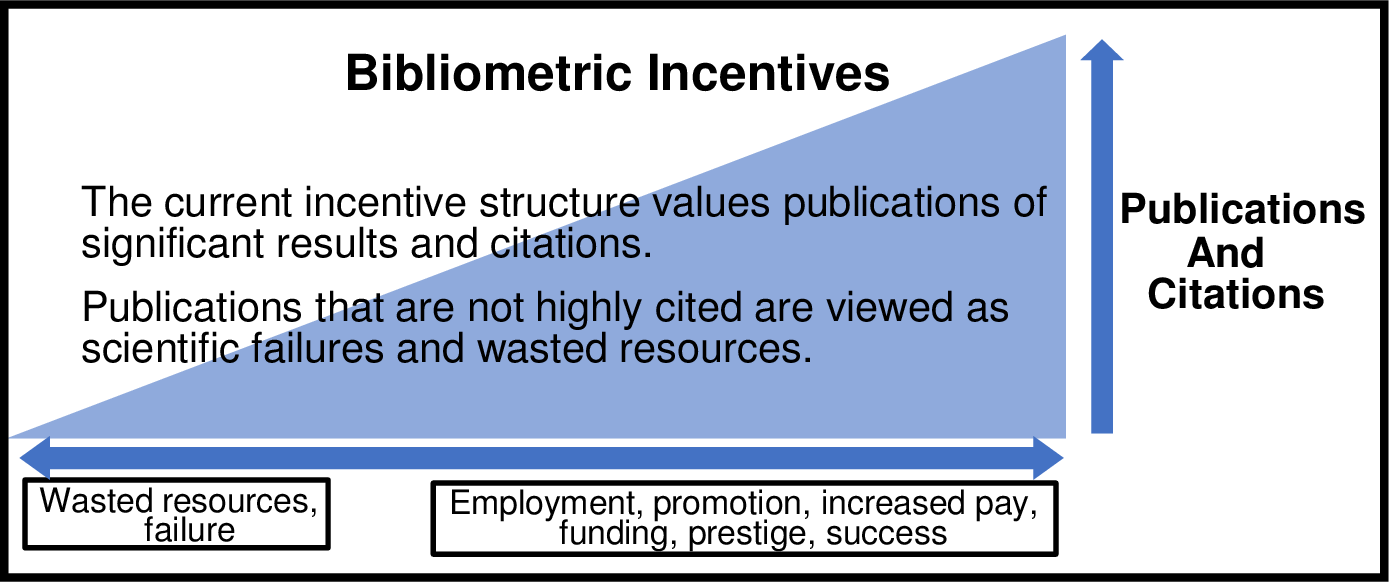
\includegraphics[height=0.5\textheight]{1.png}
        \caption{Bibliometric incentives model. \footnote{https://doi.org/10.1371/journal.pone.0195321.g001}}
    \end{figure}

\end{frame}

\begin{frame}[allowframebreaks]
    \frametitle{References}

    \bibliographystyle{apalike}
    \bibliography{references.bib}

\end{frame}

\end{document}